\chapter{Tools setup}
\label{toolsSetup}

\par
This part is a cookbook how to install all the necessary content to be able to begin development for \mbox{Cell/B.E.}
It also covers some bugs fixing as well as useful hints how to use partial SDK content.
The instruction concerning the SDK installation was based on installation on i686 machine.
But shall be the same for the other architectures since it operates on the same operating system and repository versions of third party software.

\par
The first step is installation of Fedora system.
For details see fedora official site \cite{fedorasite}.

\section{SDK installation}

As first you have to do is to download actual SDK.
Go to \url{http://www-128.ibm.com/developerworks/power/cell/ downloads.html?S_TACT=105AGX16&S_CMP=LP}.
You should download following files:

\begin{enumerate}
\item SDK 3.1 Installer
cell-install-3.1.0-0.0.noarch.rpm  (11MB), contains install script and other stuff for SDK installation.
\item SDK 3.1 Developer package ISO image for Fedora 9
CellSDK-Devel-Fedora\_3.1.0.0.0.iso  (434MB), contains rpm packages that actual SDK is composed from (SDK packages)
\item SDK 3.1 Extras package ISO image for Fedora 9
CellSDK-Extras-Fedora\_3.1.0.0.0.iso  (34MB), contains some extra packages for Fedora
\end{enumerate}

Download it wherever you want (even though in documentation is /tmp/cellsdkiso).
Lets call the folder ISODIR.
First you shall stop the YUM updater daemon.

\begin{verbatim}
/etc/init.d/yum-updatesd stop
\end{verbatim}

If this outputs: "bash: /etc/init.d/yum-updatesd: No such file or directory", you do not have any YUM updater daemon installed so you can skip this step.
Now issue following command to install required utilities for SDK installation

\begin{verbatim}
yum install rsync sed tcl wget
\end{verbatim}

Now install the downloaded installation rpm.

\begin{verbatim}
rpm -ivh ISODIR/cell-install-3.1.0-0.0.noarch.rpm
\end{verbatim}

After this step you have new stuff in \url{/opt/cell} installed. There is SDK installation script (cellsdk) located as well.
It is wrapper for YUM that manages the SDK packages.
Run it with parameter --help to see the usage.
So next step is to run it.

\begin{verbatim}
/opt/cell/cellsdk --iso ISODIR -a install
\end{verbatim}

Parameter --iso tells to use downloaded ISOs and where can be found for mounting them onto loop-back device.
Parameter -a disables agreeing licenses. Otherwise you have to write some 'yes' to agree.
Process begins with setting local YUM repositories pointing to the ISOs.
Then all default packages are installed with all their dependencies.
To check result of the installation issue

\begin{verbatim}
/opt/cell/cellsdk verify
\end{verbatim}

Now we have SDK installed. Lets continue with installation of IDE.
It consists again of packages.
Now to simplify processing packages install yumex that provides graphical interface to YUM.
And lets you simply check packages that you want.

\begin{verbatim}
yum install yumex
\end{verbatim}

To install CellIDE run yumex, go to Group View$\rightarrow$Development$\rightarrow$Cell Development Tools.
Check \textit{cellide}, that is actual IDE (Eclipse with cell concerning stuff) and \textit{ibm-java2-i386-jre}, that is Java Runtime Environment, JRE needed for running of IDE.
And click 'Process Queue'. Note: you should have the ISOs mounted onto loop-back devices.
Otherwise you get 'Error Downloading Packages' after clicking 'Process Queue'.
So you have to mount ISOs whenever you want to install package concerning Cell SDK

\begin{verbatim}
/opt/cell/cellsdk --iso ISODIR mount
\end{verbatim}

After the installation you have two new folders.
/opt/cell/ide that contains the IDE and /opt/ibm/java2-i386-50 where JRE resides.
To run the ide you have to specify folder where the JRE is (through -vm param).

\begin{verbatim}
/opt/cell/ide/eclipse/eclipse -vm /opt/ibm/java2-i386-50/jre/bin/
\end{verbatim}

\subsection{Bug fixing}
\label{XULLFIX}

If you start IDE and it crashes with unhandled exception it is probably caused by xulrunner library.
It is usually installed with Firefox3. There is following workaround:
\begin{enumerate}
\item download an older version of xulrunner

e.g. from: \url{http://releases.mozilla.org/pub/mozilla.org/xulrunner/ releases/1.8.1.3/contrib/linux-i686/ xulrunner-1.8.1.3.en-US.linux-i686-20080128.tar.gz}

\item untar to an accessible directory

Lets call it XULDIR.

\item edit the file

/opt/cell/ide/eclipse/eclipse.ini file as follows:
\begin{verbatim}
...
-vmargs
-Dorg.eclipse.swt.browser.XULRunnerPath=XULDIR
...
\end{verbatim}
\end{enumerate}
Now you should start the IDE without the crash.
Screenshot of common eclipse view is on the figure \ref{fg:eclipse}.

\begin{figure}
    \centering
    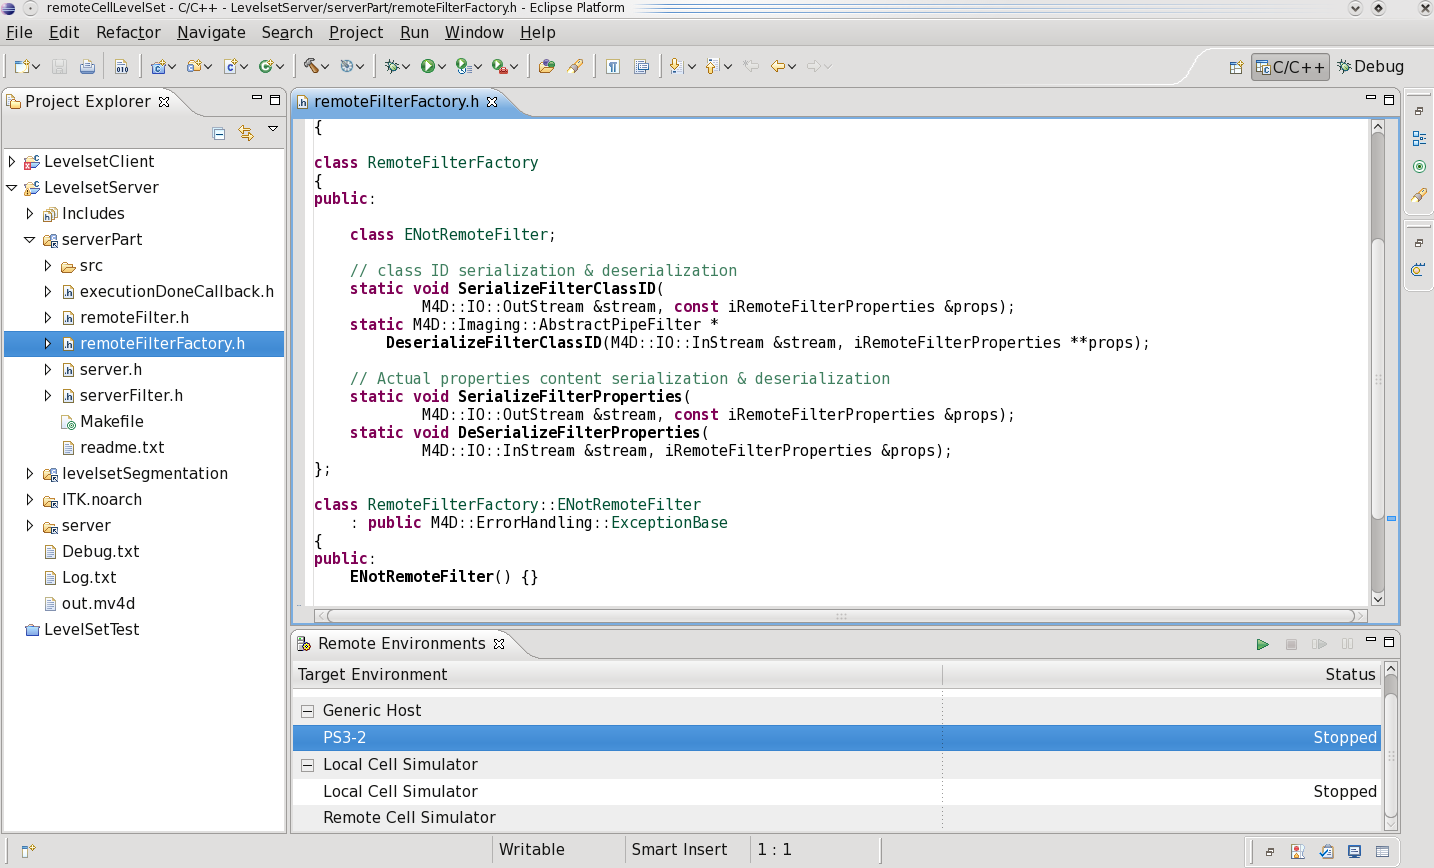
\includegraphics[width=0.95\textwidth]{data/png/eclipse}
    \caption[Screenshot of standard cellide veiw]{Sreenshot with opened source, project explorer and remote environments windows.}
    \label{fg:eclipse}
\end{figure}

\section{IBM Full-System Simulator}

The last part of development environment is IBM Full-System Simulator (systemsim).
It is not part of ISOs with SDK so you have to download it separately.
Visit \url{http://www.alphaworks.ibm.com/tech/cellsystemsim/download} and download rpm with the simulator appropriate to the platform you are currently using.
Be sure to download fedora 9 version of the simulator (cell-3.1-8.f9.*). Then install it.

\begin{verbatim}
rpm -ivh ISODIR/systemsim-cell-3.1-8.f9.i386.rpm
\end{verbatim}

Maybe some dependencies will be missing. So you have to install it. In my case it was libBLT24 and libtk8.5.

\begin{verbatim}
yum install blt tk
\end{verbatim}

Now you have simulator installed. But it has nothing to simulate.
Image with image of simulated Fedora 9 system is needed (sysroot image).
It is among SDK rpms so install it using yumex (Cell Development Tools$\rightarrow$sysroot\_image).
Now all necessary stuff is installed.
You could start the IDE and start development. But there are some bugs to fix yet.

\subsection{Bug fixing}

\par
Another issue (stack issue) is with tcl (scripting language that is used for configuration of the systemsim).
There is bug with stack size checking that causes cycling of tcl code.
To workaround this problem use ulimit command that changes default environment of Linux programs and disables the stacksize checkings.

\begin{verbatim}
ulimit -s unlimited
\end{verbatim}

\par
The last is to fix actual tcl script that manages loading the sysroot\_image (21\% issue - loading of the sysroot\_image freezes on 21\% so is not started and that's why unusable).
It is cause by wrong triggers that are triggerd when some text is output from console by the sysroot\_image loading.
There is probably triggers that wait for text from previous version of SDK that is never output in the current version.
That is why the loading freezes on 21\%.
To fix it you have to edit \url{/opt/cell/ide/eclipse/plugins/ com.ibm.celldt.simulator.profile.default_3.1.0.200809010950/ simulator_init.tcl} file.
Replace the "Welcome to Fedora Core" string with "Welcome to Fedora" and "INIT: Entering runlevel: 2" with "Starting login process".

It is useful to create starting script. That solve the stack issue and add systemsim directory to PATH (needed for running).

\begin{verbatim}
ulimit -s unlimited
PATH=/opt/ibm/systemsim-cell/bin:\$PATH
/opt/cell/ide/eclipse/eclipse -vm /opt/ibm/java2-i386-50/jre/bin
\end{verbatim}

Startup of the simulator shall finish to paused state after application of the fixes.
Screenshot of started simulator is on the figure \ref{fg:eclipseSIMStarted}.

\begin{figure}
    \centering
    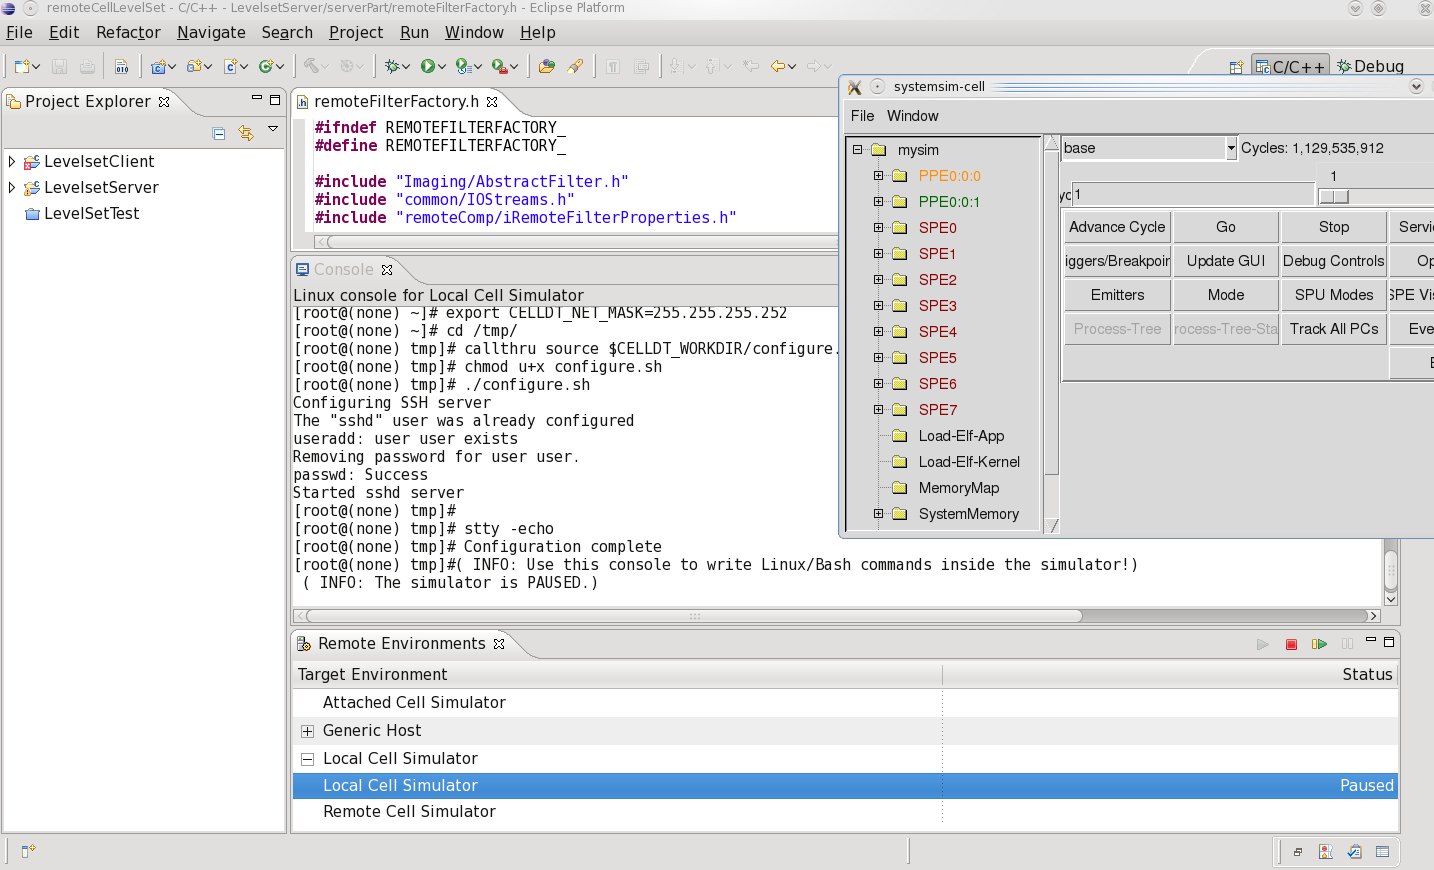
\includegraphics[width=0.95\textwidth]{data/png/eclipseSIMStarted}
    \caption[Cellide with started simulator]{Screenshot of Eclipse cellide after simulator startup. Remote environments window contain Local Cell Simulator item that is in paused state. Above this window is simulator console with few last outputs. On the upper left side is part of simulator control window.}
    \label{fg:eclipseSIMStarted}
\end{figure}

\subsection{Installation of libraries into sysroot\_image}

Because sysroot\_image is provided as image of installed Fedora 9 without any \mbox{Cell/B.E.} libraries so next step is to install them into sysroot\_image.

\begin{verbatim}
/opt/cell/cellsdk_sync_simulator install
\end{verbatim}

This shell script installs all rpms for ppc and ppc64 platforms that finds in \url{/tmp/cellsdk/rpms}.
By default these rpms are copied into \url{/tmp/cellsdk/rpms} during the install process.
If they are not still there (or in installed subdirectory) you have to copy them by hand from ISOs (note: ISOs has to be mounted).

\begin{verbatim}
cp \
/opt/cell/yum-repos/CellSDK-Devel-Fedora/rpms/*.{ppc,ppc64}.rpm\
/tmp/cellsdk/rpms
\end{verbatim}

\subsection{Copying content into sysroot\_image}

Sysroot\_image is common binary image that can mounted and thus some additional content copied into.
This is useful when extra library that are not part of the default image need to be used.
In my case that was some boost libraries. So to mount the sysroot\_image issue:
\begin{verbatim}
mount -o loop /opt/ibm/systemsim-cell/images/cell/sysroot_disk\
<your mount point>
\end{verbatim}
And then copy whatever you want.

\subsection{Simulator hints}

\par
You can ssh to running simulator. It is better to use real bash that the console within IDE.
You have all the bash advantages like command and path completion available in contrast to 'text mode' of the IDE console.

\par
Sometimes root user is needed for an operation performed in the simulator.
Its password should be disabled.
It can be done when sysroot\_image is mounted.
Under host machine root account the \url{<sysroot_image_mount_point>/etc/passwd} file should be edited.
The first line is the root's so deletion of '*' character from the second field (after the second ':' character) will disable the root's password.
Note that this action must be performed when the simulator is not running otherwise the changes will be overwritten by the simulator.

\section{Using examples}

Examples are installed into /opt/cell/sdk/src as tarball.
So you have to untar each you want to use.
It is good to start with examples and tutorial sources.
Each folder has its own makefile that manages makefiles in its sub folders.
So you can call only the top level one to build all projects in sub folders or any from the sub folders to build particular projects.

It is convenient to use the sample sources in CellIDE where you can build it as well and create run/debug configuration for running within cell environment.
To use the example code (for example \url{/opt/cell/sdk/src/tutorial/simple}) create new c++ makefile project.
Click right button on it to get into properties.
C/C++ general tab $\rightarrow$ Paths and Symbols $\rightarrow$ Source location.
Here you have to add the folder with the sources (\url{/opt/cell/sdk/src/tutorial/simple}) by 'create / link folder' button $\rightarrow$advanced $\rightarrow$ link to folder in filesystem.
Now you have two folders in list. The first one is the original, created during project creation and the other newly linked folder with the source.
You can delete the original one since you are not going to use it.
Next is necessary to set up 'Build directory' to tell the IDE where shall search for makefile.
It is C/C++ Build tab. Use 'Workspace' button to specify the folder because it will use workspace\_loc variable and thus independent on exact location on filesystem.

\section{Tuning memory usage on PS3}
\label{ps3MemoryUsage}

PS3 has only 256MB RAM memory and even not the whole is visible for operating system.
This is very small amount for operating system and programs together.
When install fedora system with default state and boot up it, the amount of remaining free memory is about 10MB.
It is insufficient for either debugging and compilation.
So some of resources has to be switched off.
Our PS3s are accessed remotely via ssh so there is no need for X server.
So this is the first you can turn off. This is performed by change of runlevel from 5 to 3.
Run level setting is in \url{/etc/inittab} file. So change in line
\begin{verbatim}
"id:5:initdefault:"
\end{verbatim}
the 5 to 3.

\par
Another resource are services.
Here you have to consider if the service you want to turn off is really unnecessary.
In Our PS3 NeworkManger and Wireless supplicant was turn off.
NOTE: when you turn off network manager, you have to turn on network service otherwise the networking will not run properly.
For service management within ssh console \url{/usr/sbin/ntsysv} manager is quite useful.
After disabling all unnecessary services we got about 130MB of free space.

\par
Yellow dog distributions goes even beyond. They can access another 256MB in PS3 locked for graphics.
Special device is created and the graphic memory is the used as a swap partition. For details see \url{http://us.fixstars.com/products/ydl/}.

\section{Performance tools}

Information about packages concerning performance tools can be obtained by:
\begin{verbatim}
yum groupinfo "Cell Performance Tools"
\end{verbatim}
If they are not already installed issue following command to install them.
\begin{verbatim}
yum groupinstall "Cell Performance Tools"
\end{verbatim}

\section{Visual Performance Analyser - VPA}

Another useful tool is VPA. It is not part of SDK so it should be downloaded separately.
Visit \url{http://www.alphaworks.ibm.com/tech/vpa} for details.
After installing (actually unpacking) the downloaded file similar fix in ini file to eclipse.ini file (see paragraph \ref{XULLFIX}) should be done to run the VPA correctly.

\section{\mbox{Cell/B.E.} cross compilation}

When crosscopiling a \mbox{Cell/B.E.} program which uses lot of third party libraries it is good idea to share some folders on actual \mbox{Cell/B.E.} machine.
There is not necessary to copy different architecture stuff to the machine where the cross compilation is performed as we did.
In our case it was boost and ITK libraries and we performed crosscompilation for \mbox{Cell/B.E.} on a i686 machine.
We wanted to use repository versions of the \mbox{Cell/B.E.} resp. ppc64 libraries on our i686 machine.
So the first thing we tried was to install appropriate packages of different architecture.
But we have not found a way how to do it.
Every try has failed due to architecture mismatch.
So we believe that mounting remote \mbox{Cell/B.E.} machine shared folders is the only way how to use repository content directly and avoid copying different architecture content.
